% !TEX root = sum1.tex
\section{Problem Formulation}
In this section, we give the description of the problem, then present the deterministic and stochastic formalution.

\subsection{Problem Description}
% In this section we present the model that generates seat assignment under deterministic demands.

First, we will introduce some preliminary knowledge about our problem as follows.

Consider a set of groups to be assigned to a set of seats. For illustration, we consider the layout as $N$ rows, each row with $S_{j}$ seats, $j = 1, \ldots, N$. 

% But our model and formulation allow for a more general layout of the seats. 
According to the epidemic prevention requirements, the customers from the same group can sit together, while different groups should sit with social distancing. 
Suppose that each group has to leave one seat to maintain social distancing from the adjacent groups and different rows have no effect on each other, i.e., a person from one group can sit directly behind a person from another group.

% Considering the actual situation, social distancing is one seat in our paper 
Let the $i-$th group type contain $i$ people. To implement the social distancing in the seat assignment, we add one to the original size of each group as the new size of the group and one dummy seat to each row. Take $s_{i} = i + 1$, $L_{j} = S_{j} +1$, $s_{i}$ is the new size of group type $i$ and $L_{j}$ is the length of row $j$.

Then we can illustrate the seat assignment for one row below. 

\begin{figure}[ht]
    \centering
    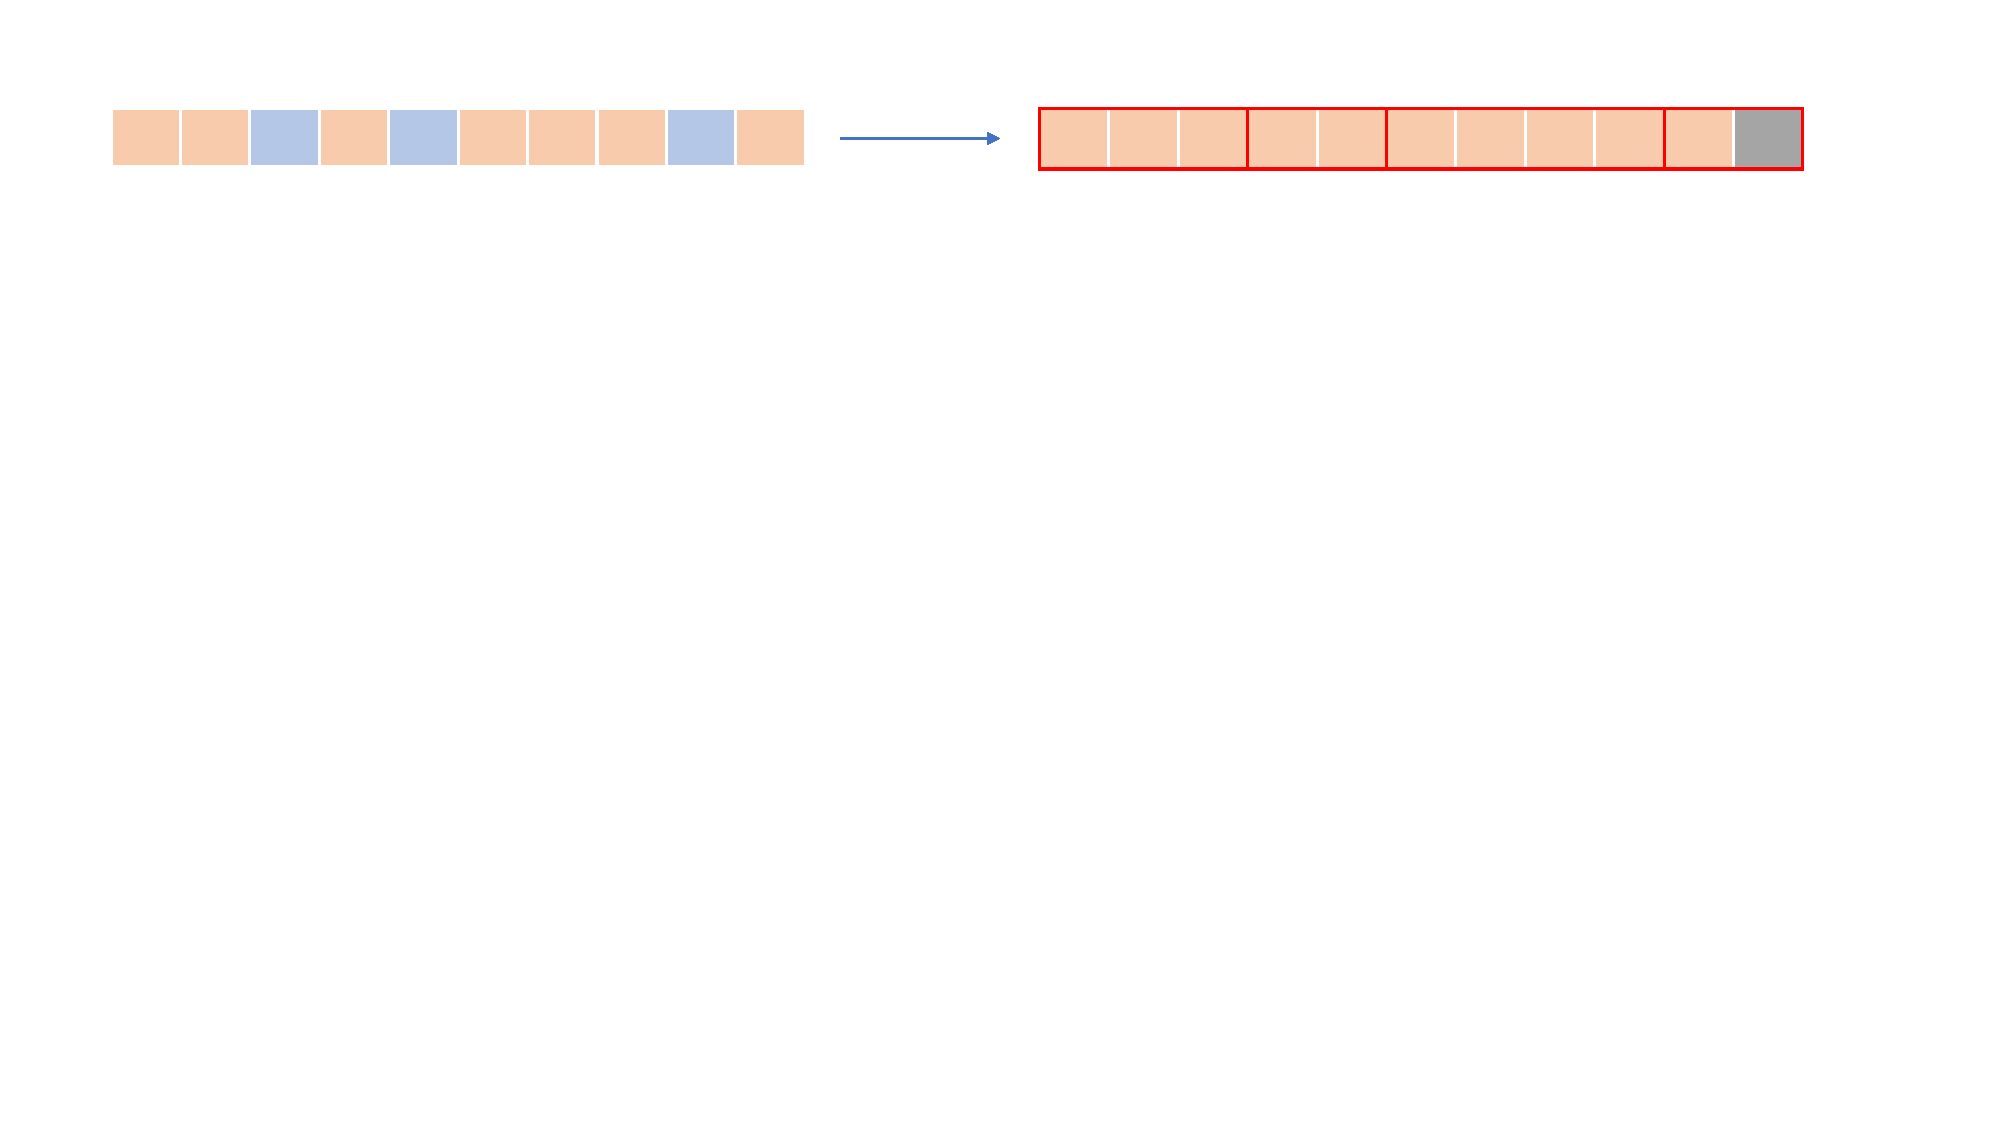
\includegraphics[width = 0.8\textwidth]{./Figures/dummy_seat.pdf}
    \caption{Problem Conversion}
\end{figure}

On the left side, the blue squares stand for the empty seats as the social distancing. The orange squares represent the seats sat by the groups. 
On the right side, one dummy seat is added at the end of the row. The orange squares surrounded by the red line are the seats taken by groups.

In this way, the social distancing will be integrated by solving this new seat assignment problem.

% The number of all seats in each row is called the length of the row.

\subsection{Deterministic Model}
When given a deterministic demand, for example, $(d_1, d_2, d_3, d_4) = (3,5,7,6)$, where $d_i$ indicates the number of $i$-th group type. 

To accommodate as many as people possible in the fixed rows, the IP formulation can be shown below:
\begin{equation}\label{deter_upper}
    \begin{aligned}
      \max \quad & \sum_{j =1}^{N} \sum_{i = 1}^{m} (s_i -1) x_{ij} \\
      \text {s.t.} \quad & \sum_{i = 1}^{m} s_i x_{ij} \leq L_{j}, j=1,\ldots,N \\
      & \sum_{j =1}^{N} x_{ij} \leq d_{i}, i=1,\ldots,m \\
      & x_{ij} \geq 0, \text{integer}~ i=1,\ldots,m, j=1,\ldots,N.
    \end{aligned}
\end{equation}

$m$ indicates the number of group types. $x_{ij}$ indicates the number of group type $i$ placed in row $j$.

When we need to consider the lower bound of the demand which represents the groups must be assigned seats, we can add a new constraint $\sum_{j =1}^{N} x_{ij} \geq d_{i}^{l}, i=1,\ldots,m$ in \eqref{deter_upper}, $d_{i}^{l}$ is the number of group type $i$ we have accepted.

When a lower or upper bound is not needed, the corresponding constraint can be removed. Because the ratio of value to capacity is monotone for the size of groups, the solver can quickly solve this deterministic formulation without many branching operations.

% when the capacity allows accepting the groups from large to small as many as possible will give an optimal solution.


% Before that, we give the deterministic model with a lower bound and upper bound of demand as below,
% \begin{equation}\label{deter_lower_upper}
%     \begin{aligned}
%       \max \quad & \sum_{j =1}^{N} \sum_{i = 1}^{m} (s_i -1) x_{ij} \\
%       \text {s.t.} \quad & \sum_{i = 1}^{m} s_i x_{ij} \leq L_{j}, j=1,\ldots,N \\
%       & \sum_{j =1}^{N} x_{ij} \geq d_{i}^{l}, i=1,\ldots,m \\
%       & \sum_{j =1}^{N} x_{ij} \leq d_{i}, i=1,\ldots,m \\
%       & x_{ij} \geq 0, \text{integer},  i=1,\ldots,m, j=1,\ldots,N.
%     \end{aligned}
%   \end{equation}

% $d_{i}^{l}$ is the lower bound of the demand. (It can be the number of group type $i$ we have accepted.)
% $d_{i}^{u}$ is the upper bound of the demand. (deterministic demand)


% Why is it easy to solve this IP?

% If the ratio is the same for the groups, IP will use more branches to obtain an optimal solution.

% $[24,28,8,9]$ 10 rows.
% Total loss: 60; loss of the largest pattern: 5.


